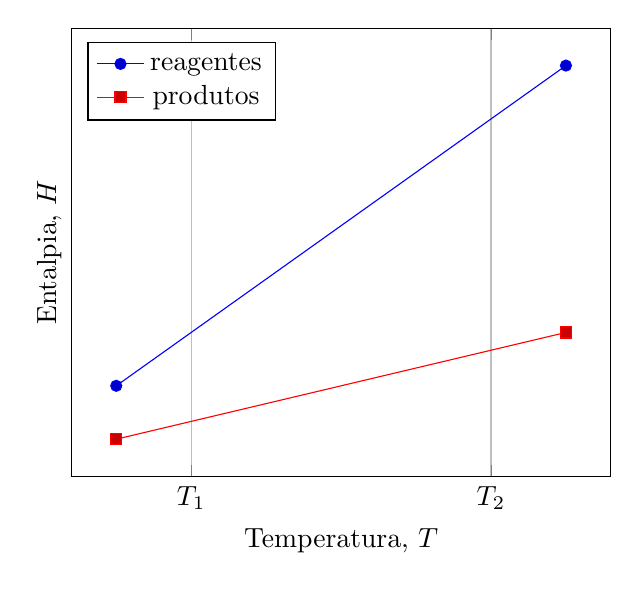
\begin{tikzpicture}
    \begin{axis}
        [
            grid = major,
            xlabel = {Temperatura, $T$},
            ylabel = {Entalpia, $H$},
            xmajorgrids,
            ytick=\empty,  
            legend pos = north west, 
            xtick={1.5,3.5},
            xticklabels={$T_1$,$T_2$},
        ]
    \addplot coordinates
        {
            (1,2)
            (4,8)
        };
    \addplot coordinates
        {
            (1,1)
            (4,3)
        };
    \legend{reagentes, produtos}
    \end{axis}
\end{tikzpicture}